% GENERATED by benchmarks/scripts/paper.py -- do not edit.
% artifact:   fig_vs_cpp (figure)
% result set: current
% commit:     18d0f83627b5
% host:       a2
% measured:   2026-09-12
% inputs:     sha256:51d37586d0e48420
% provenance: paper/generated/PROVENANCE.md#fig_vs_cpp
%
\begin{figure}[tb]
\centering
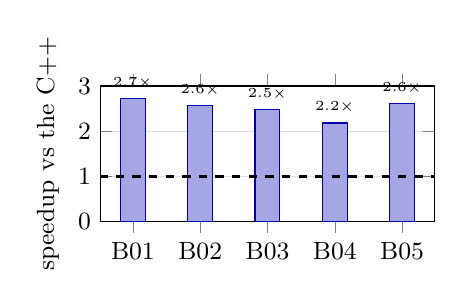
\begin{tikzpicture}
\begin{axis}[
  width=0.48\textwidth, height=3.3cm, ybar, bar width=9pt, ymin=0,
  xtick={0,1,2,3,4},
  xticklabels={{B01},{B02},{B03},{B04},{B05}},
  x tick label style={font=\small}, y tick label style={font=\small},
  ylabel={speedup vs the C++}, ylabel style={font=\small},
  enlarge x limits=0.12, ymajorgrids, grid style={gray!25},
  nodes near coords, nodes near coords style={font=\tiny},
  point meta=explicit symbolic,
]
\addplot[draw=blue!70!black, fill=blue!70!black!35] coordinates {(0,2.74) [2.7$\times$] (1,2.58) [2.6$\times$] (2,2.49) [2.5$\times$] (3,2.19) [2.2$\times$] (4,2.63) [2.6$\times$]};
\draw[black,dashed,thick] (axis cs:-0.5,1) -- (axis cs:4.5,1);
\end{axis}
\end{tikzpicture}
\hfill
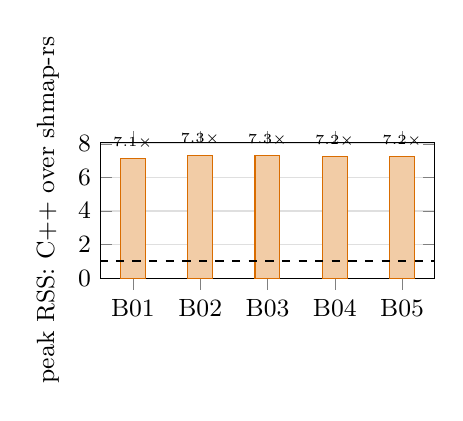
\begin{tikzpicture}
\begin{axis}[
  width=0.48\textwidth, height=3.3cm, ybar, bar width=9pt, ymin=0,
  xtick={0,1,2,3,4},
  xticklabels={{B01},{B02},{B03},{B04},{B05}},
  x tick label style={font=\small}, y tick label style={font=\small},
  ylabel={peak RSS: C++ over shmap-rs}, ylabel style={font=\small},
  enlarge x limits=0.12, ymajorgrids, grid style={gray!25},
  nodes near coords, nodes near coords style={font=\tiny},
  point meta=explicit symbolic,
]
\addplot[draw=orange!85!black, fill=orange!85!black!35] coordinates {(0,7.10) [7.1$\times$] (1,7.33) [7.3$\times$] (2,7.30) [7.3$\times$] (3,7.25) [7.2$\times$] (4,7.25) [7.2$\times$]};
\draw[black,dashed,thick] (axis cs:-0.5,1) -- (axis cs:4.5,1);
\end{axis}
\end{tikzpicture}
\caption{The two headline results, per benchmark, single-threaded on both sides: wall-clock speedup over the C++ (top) and how many times less peak memory the port uses (bottom). The dashed line is parity.}
\label{fig:vscpp}
\end{figure}
